\def\CTeXPreproc{Created by ctex v0.2.9, don't edit!}
%\documentclass{beamer}
\documentclass[%handout,
xcolor=pdftex]{beamer}
\mode<presentation> {
  \usetheme{Warsaw}
  \setbeamercovered{transparent}
}
\let\Tiny=\tiny
\usetheme{Singapore}
\usecolortheme{dolphin}
\usepackage{amsmath}
\usepackage{textcomp}
\usepackage{amssymb}
\usepackage{amsthm}
\usepackage{graphicx}
\usepackage{color}
\usepackage{lipsum}
\usepackage{hyperref}
\usepackage{multirow}
\usepackage{bm}

\usepackage{mathtools}
\DeclarePairedDelimiter\ceil{\lceil}{\rceil}
\DeclarePairedDelimiter\floor{\lfloor}{\rfloor}


%\setbeamertemplate{headline}{}
\setbeamertemplate{footline}[page number]
\newcommand\Fontvi{\fontsize{9pt}{8}\selectfont}
\newcommand\Fontvii{\fontsize{7pt}{8}\selectfont}
\newcommand{\backupbegin}{
   \newcounter{finalframe}
   \setcounter{finalframe}{\value{framenumber}}
}
\newcommand{\backupend}{
   \setcounter{framenumber}{\value{finalframe}}
}\newtheorem{proposition}{Proposition}
\title{Unit 6: Exploratory Data Analysis II}
\author[STAT 5170: Applied Time Series, Unit 6]{Taylor R. Brown PhD}
\institute{Department of Statistics, University of Virginia}
\date{Spring 2020}

\AtBeginSubsection[] {
  \begin{frame}<beamer>{Outline}
    \tableofcontents[currentsection,currentsubsection]
  \end{frame}
}

\begin{document}


\frame{\titlepage}


\begin{frame}
\frametitle{Readings for Unit 6}

Textbook chapter 2.2 (page 66).

\end{frame}


\begin{frame}
\frametitle{Last Unit}
\begin{enumerate}
\item Detrending
\item Differencing for Stationarity
\item Backshift Operator
\end{enumerate}
\end{frame}

\begin{frame}
\frametitle{This Unit}
\begin{enumerate}
\item Periodic functions
\item Exploratory data tools to access frequency
\end{enumerate}
\end{frame}

\begin{frame}
\frametitle{Motivation}

We've already seen how we can use differencing to obtain stationary processes.  We are assuming that our observations can be written in the form
\begin{equation} \label{eq:basic}
x_t=\mu_t+y_t
\end{equation}

where $\mu_t$ is some function of time and $y_t$ is a
stationary process. What if $\mu_t$ were not a
trend, but a periodic function?

\end{frame}

\section{Periodic Functions}
\frame{\tableofcontents[currentsection]}

\begin{frame}
\frametitle{Setup}

A basic type of \textbf{periodic}
function would be
$$
\mu_t=A cos( 2 \pi \omega t + \phi),
$$

where

\begin{itemize}
\item $A$: amplitude,
\item $\omega$: frequency,
\item $1/\omega$: period,
\item $\phi$: phase.
\end{itemize}

Note that a cosine function is equal to a sine function for some phases, e.g. $cos(2 \pi \omega t)  = sin(2 \pi \omega t + \frac{\pi}{2})$.

\end{frame}

\begin{frame}
\frametitle{Setup}

For now we assume that $y_t$ in model (\ref{eq:basic}) is white noise.  Model (\ref{eq:basic}) is now written as

\begin{equation} \label{eq:periodic}
x_t=A cos( 2 \pi \omega t + \phi)+w_t.
\end{equation}

\end{frame}

\begin{frame}
\frametitle{Setup}

We could try to use non-linear least squares to fit $A$,
$\omega$ and $\phi$. Recall
the identity $cos(\alpha+\beta)=cos(\alpha)cos(\beta) -
sin(\alpha)sin(\beta)$. Thus, we can rewrite model (\ref{eq:periodic}) as

\begin{eqnarray}
x_t &=&  \underline{\hspace{80 mm}} \nonumber \\
    &=&  \underline{\hspace{80 mm}} \nonumber \\
    &=&  \underline{\hspace{80 mm}}
\end{eqnarray}

\end{frame}

\begin{frame}
\frametitle{Frequencies}

In many settings, certain frequencies are natural.  For example, in monthly data a frequency,  $\omega$, of 1/12 (corresponding to a period of 12) is quite natural.  We may want to remove a periodic signal by fitting
$$
x_t= \beta_1 cos( 2 \pi /12 \  t )+\beta_2 sin( 2 \pi /12 \  t )+w_t
$$

and then analyzing the residuals to understand $w_t$. This is regular regression by treating $cos(2\pi/12 \ t)$ and $sin( 2 \pi /12 \  t )$ as the \textbf{predictor variables} and we may use
OLS to estimate $\beta_1, \beta_2$.

\end{frame}

\begin{frame}
\frametitle{OLS Estimation}

There are solutions for the estimates of these
parameters.

\begin{eqnarray*}
\hat{\beta}_1 &=& \frac{2}{n} \sum_{t=1}^n x_t cos( 2 \pi \frac{1}{12} t ).\\
\hat{\beta}_2 &=& \frac{2}{n} \sum_{t=1}^n x_t sin( 2 \pi \frac{1}{12} t ).
\end{eqnarray*}

\end{frame}

\section{Exploratory Data Tools to Access Frequency}
\frame{\tableofcontents[currentsection]}

\begin{frame}
\frametitle{Choosing Frequency}

If we do not have an intuition regarding the frequency, we could try various regressions with different frequencies, $\omega$, of the form $\frac{j}{n}$ for $j=1,\ldots,\floor{\frac{n}{2}}$.  This guarantees evenly spaced frequencies from zero to 0.5. The parameters can be estimated by

\begin{eqnarray*}
\hat{\beta}_1(j/n) &=& \frac{2}{n} \sum_{t=1}^n x_t cos( 2 \pi t j/n ).\\
\hat{\beta}_2(j/n) &=& \frac{2}{n} \sum_{t=1}^n x_t sin( 2 \pi t j/n  ).
\end{eqnarray*}

\end{frame}

\begin{frame}
\frametitle{Choosing Frequency}

We then obtain the value of $\hat{\beta}_1^2(j/n)+\hat{\beta}_2^2(j/n)$ for all these frequencies, which can be interpreted as the amount of variation at a certain frequency. A measure of the presence of a frequency oscillating at a frequency of $j/n$ would be

\begin{equation*}
P(j/n) = \hat{\beta}^2_1(j/n) + \hat{\beta}^2_2(j/n).
\end{equation*}

The quantity $P(j/n)$ is called the \textbf{scaled periodogram}. 

% Note that:

\vspace{30mm}

\end{frame}

\begin{frame}
\frametitle{Exploratory Data Tools}

\begin{itemize}
\item Periodogram (as described in the previous slide). Works for stationary time series.
\item ACF plot. Recall that the ACF is a correlation of lags; this makes sense in a stationary time series as well.
\item Lag plot. Useful with \textbf{periodic} data--each scatter plot has $x_t$ on the y-axis and $x_{t-h}$ on the x-axis.
\end{itemize}

\end{frame}

\section{Worked Example}
\frame{\tableofcontents[currentsection]}

\begin{frame}
\frametitle{Example: Australian Unemployment}

Let's look at these techniques with an example. The data consist of Australian unemployment numbers recorded monthly from Feb 1978 to Aug 1995 (in thousands).

\end{frame}

\begin{frame}
\frametitle{Example: Australian Unemployment}

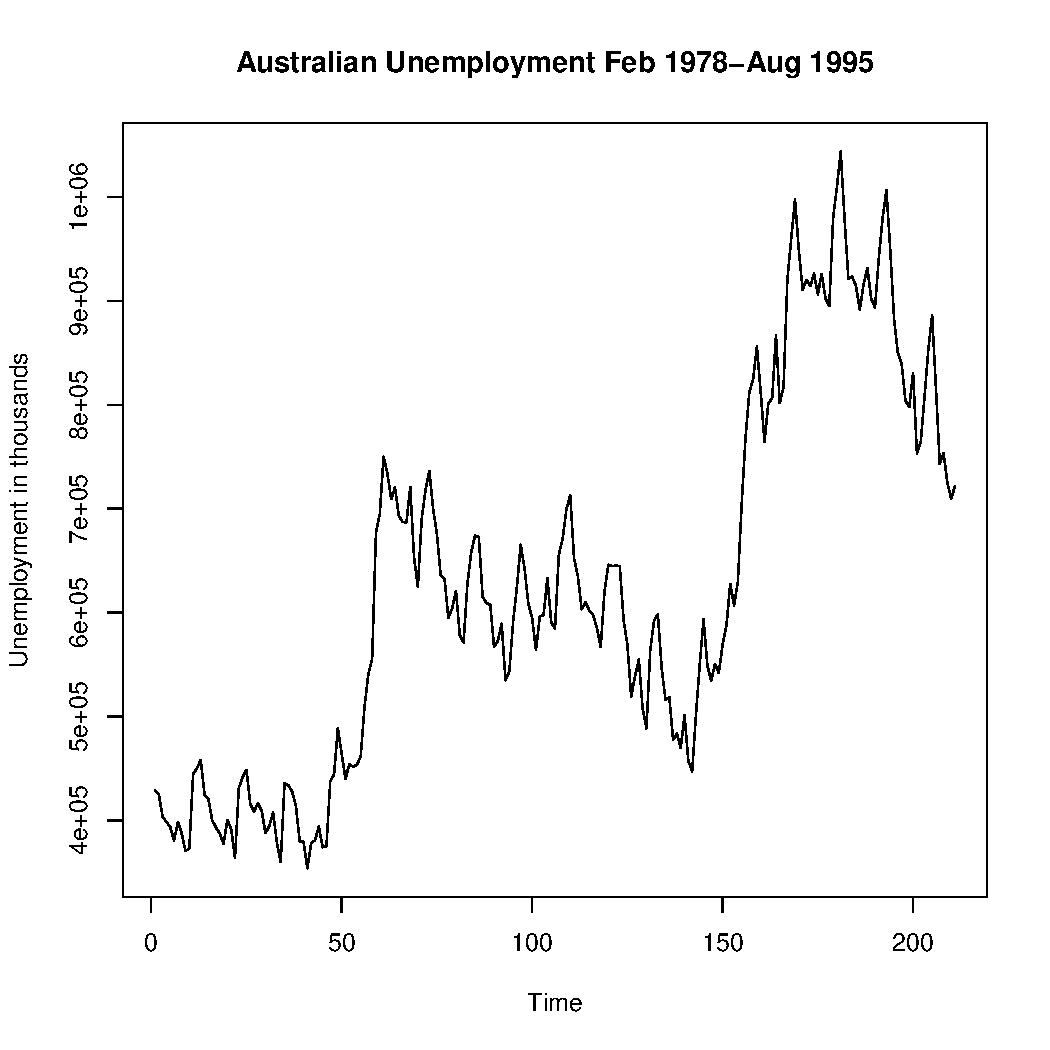
\includegraphics[width=100mm, height=60mm]{pics/auemp.pdf}

\textbf{Question}: Do the data look stationary?

\end{frame}

\begin{frame}
\frametitle{Example: Australian Unemployment}

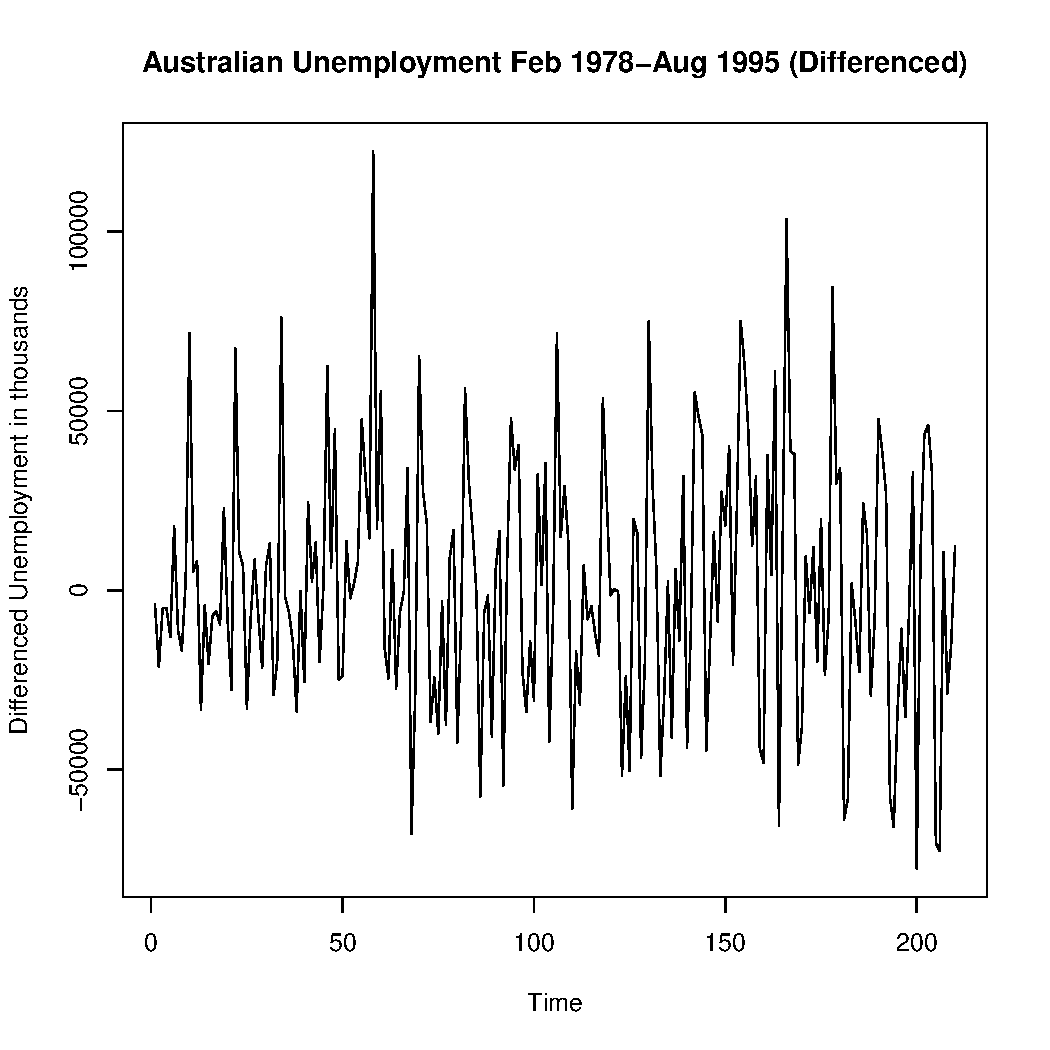
\includegraphics[width=100mm, height=80mm]{pics/dauemp.pdf}

\end{frame}

\begin{frame}
\frametitle{Example: Australian Unemployment}

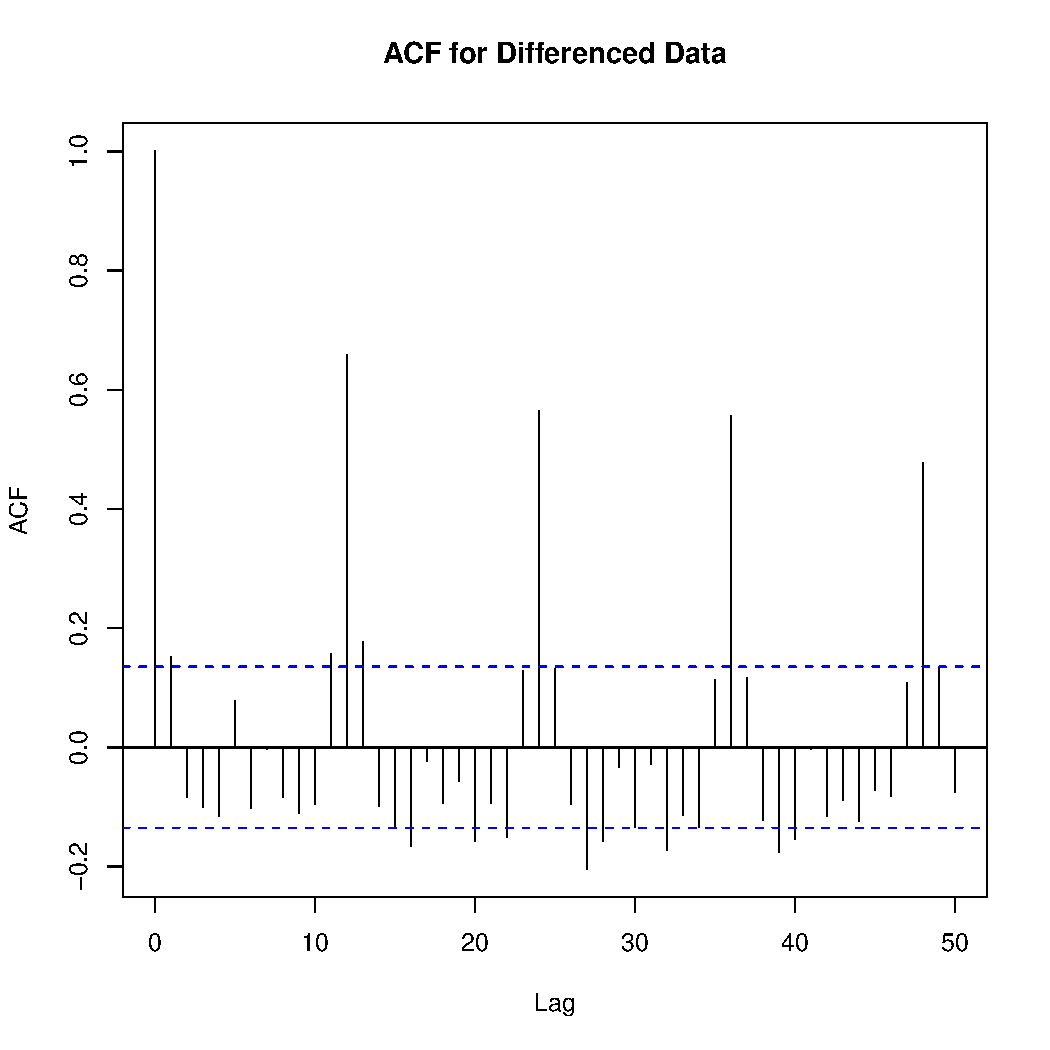
\includegraphics[width=100mm, height=60mm]{pics/acfdauemp.pdf}

\textbf{Question}: What does the ACF indicate?

\end{frame}

\begin{frame}
\frametitle{Example: Australian Unemployment}

\includegraphics[width=100mm, height=60mm]{pics/lagplotdauemp.pdf}

\textbf{Question}: What do the lag plots indicate?

\end{frame}

\begin{frame}[fragile]
\frametitle{Example: Australian Unemployment}

\begin{verbatim}
auemp<-ts(scan("unemploy.dat", skip=1))
dauemp<-ts(diff(auemp))

plot(auemp)
plot(dauemp)
acf(dauemp,50)
lag.plot(dauemp, lags=12, diag=F)
\end{verbatim}

\end{frame}

\begin{frame}
\frametitle{Example: Australian Unemployment}

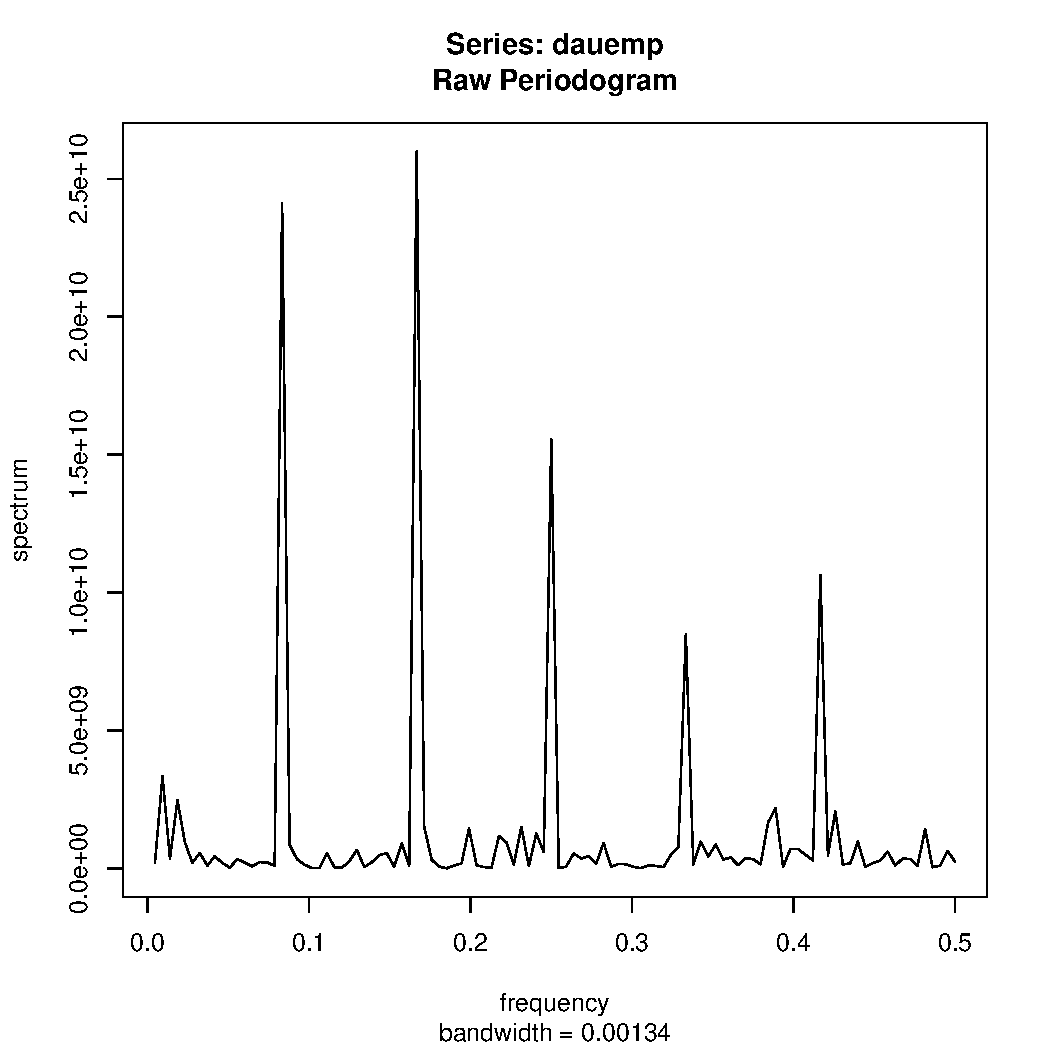
\includegraphics[width=100mm, height=60mm]{pics/perioddauemp.pdf}

\textbf{Question}: What does the periodogram indicate?

\end{frame}

\begin{frame}[fragile]
\frametitle{Example: Australian Unemployment}

\begin{verbatim}
temp<-spec.pgram(dauemp, taper=0, log="no")

freq<-temp$freq[temp$spec>5e9]
freq
[1] 0.08333333 0.16666667 0.25000000 0.33333333 0.41666667
\end{verbatim}

\end{frame}


\begin{frame}
\frametitle{Example: Australian Unemployment}

Let's perform regression at these 5 peaks.

\includegraphics[width=100mm, height=60mm]{pics/fitteddauemp.pdf}

\end{frame}

\begin{frame}[fragile]
\frametitle{Non-Stationary Residuals}

\textbf{Question}: If the residuals exhibit non-stationarity, what does that suggest?

\end{frame}

\begin{frame}[fragile]
\frametitle{Example: Australian Unemployment}

\begin{verbatim}
t=1:length(dauemp)
c1<-cos(2*pi*t*freq[1])
s1<-sin(2*pi*t*freq[1])
c2<-cos(2*pi*t*freq[2])
s2<-sin(2*pi*t*freq[2])
c3<-cos(2*pi*t*freq[3])
s3<-sin(2*pi*t*freq[3])
c4<-cos(2*pi*t*freq[4])
s4<-sin(2*pi*t*freq[4])
c5<-cos(2*pi*t*freq[5])
s5<-sin(2*pi*t*freq[5])
fit<-lm(dauemp~c1+s1+c2+s2+c3+s3+c4+s4+c5+s5)
\end{verbatim}

\end{frame}

\begin{frame}[fragile]
\frametitle{Example: Australian Unemployment}

\begin{verbatim}
fitted<-ts(fit$coef[2]*c1+fit$coef[3]*s1+fit$coef[4]
*c2+fit$coef[5]*s2+fit$coef[6]*c3+fit$coef[7]
*s3+fit$coef[8]*c4+fit$coef[9]*s4+fit$coef[10]
*c5+fit$coef[11]*s5)

par(mfrow=c(3,1))
plot(fitted, ylim=c(miny,maxy), main="Fitted Values")
plot(ts(fitted-dauemp), ylim=c(miny,maxy), main="Residuals")
acf(ts(fitted-dauemp), main="ACF for Residuals")
\end{verbatim}

\end{frame}




\begin{frame}
\frametitle{Recap}

To recap, we consider model (\ref{eq:basic}) which take the form

$$
x_t=\mu_t+y_t
$$

where $\mu_t$ is a either a polynomial or periodic function, and $y_t$ is a zero mean stationary process.

\end{frame}

\begin{frame}
\frametitle{Recap}

If $\mu_t$ is polynomial, we can

\begin{itemize}
\item Difference to coerce stationarity.
\item Use least squares regression, if estimating $y_t$ is the goal.
\end{itemize}

If $\mu_t$ is periodic, we can use the periodogram to identify prevalant frequencies.

\end{frame}


\end{document} 